\chapter{Compiling the Corpus}
\label{chap:compiling}
\section{Introduction}

The corpus at hand incorporates the press releases published by the Canton of \Gls{graubuenden}. 
These press releases are a means of the cantonal government to publish news and information about topics such as politics, economy, health and culture. 
Graubünden, which is made up of German speaking, Italian speaking and Romansh speaking regions, is the only trilingual canton in Switzerland. 
As such, virtually all press releases are published in these three languages.
This trilingual setting lends itself to be collected to a parallel trilingual corpus.

\section{Collecting the Data}
At first, I contacted the \emph{\Gls{standeskanzlei}} (\enquote{State Chancellery of Grisons}) which is the \enquote{the general administrative authority for questions of office, coordination and liaison with the cantonal parliament (\enquote{Grosser Rat}), government and cantonal administration} \autocite{staka}. 
The \emph{\Gls{standeskanzlei}}, with its \emph{Übersetzungsdienst} (\enquote{Translation service}), is responsible for translating documents in service of the canton.
I was hoping to receive the data directly from them---after all, we are not talking about private or commercial data, but about public translation work financed with taxpayers' money.

I spoke to Mr.~Mirco Frepp from the communication sevices (\emph{Kommunaktionsdienst}), which, although very friendly, had to inform me that it would be impossible for me to receive the data. 
The explanation was that the documents are not saved locally somewhere, but are saved in a database. 
The documents are extracted from the database and are generated as ad-hoc HTML documents whenever the website is accessed. 
It was also not possible to receive a dump of the database.

\section{Web Scraping}
Not being able to receive a dump of the database meant I had to scrape the canton's website, extract the relevant content from the HTML files and construct my own database. In order to achieve this, I wrote a series of Python scripts that would take care of these tasks. 
All the scripts can be found on my GitHub repository\footnote{\url{https://github.com/eyldlv/de_rm_it_corpus}}. 
The scripts relevant for the database building are saved under the folder \texttt{corpus\_builder}.

\begin{figure}
\dirtree{%
.1 corpus\_builder.
.2 corpus\_builder.
.3 access\_db.py.
.3 create\_corpus.py.
.2 web\_scraper.
.3 test\_web\_scraper.py.
.3 web\_scraper.py.
}

\caption{Directory tree of \texttt{corpus\_builder}}
\end{figure} 
\subsubsection{Web Scraper}
\label{subsubsec:web-scraper}
The script \texttt{web\_scraper.py} goes to the index web page for each year and language. 
This page contains the links pointing to all the press releases that were released that year. 
It collects all those links, and then downloads the HTML from each link. 
The HTML pages are saved in separate folders for each year. 
The filenames have the following format: \texttt{year\_file-id\_language}, e.g., \texttt{1997\_12924\_DE.html}. 
The file-id is taken from the URL and will be later used to align the documents. 


\begin{figure}[ht]
\dirtree{%
.1 html.
.2 1997.
.3 1997\_12924\_DE.html.
.3 1997\_12936\_IT.html.
.3 {...}.
.2 1998.
.2 1999.
.2 {...}.
.2 2022.
.3 2022\_2022010301\_DE.html.
.3 2022\_2022010301\_IT.html.
.3 2022\_2022010301\_RM.html.
.3 {...}.
}
\caption{Directory scheme for saving the HTML files}
\label{fig:html-scheme}
\end{figure} 

Since the script makes many requests to the website, one has to anticipate that the server might stop responding, which will result in a request time-out.  This means the script will have to be run a couple of times.
To avoid downloading HTML pages that were already downloaded, the script will skip and press releases that already exist locally, providing the file size is greater than 0 bytes.
This way, the script can also be run at a later stage, after additional new press releases were published, in order to update the local repository.
To make sure the local copy of the press releases is complete, the script can simply be run repeatedly until a message is printed to the console that no new press releases were downloaded. 

By default, the script will download the press releases for the entire year range (1997 to the current year) and in all three languages. 
This can be limited by using the following optional arguments:
\begin{itemize}
	\item \texttt{-{}-year} -- limit the scraping to a year or to a range of years separated by a comma, e.g., \texttt{-{}-year 2022} or \texttt{-{}-year 2020,2022}
	\item \texttt{-{}-lang} -- limit the scraping to one or more languages (comma separated), e.g., \texttt{-{}-lang de,it}
\end{itemize}

\section{Building the Corpus}
All the scripts responsible for building the corpus can be found under the folder \texttt{corpus\_builder}.

\subsection{HTML Parsing}
After the creation of a local copy of the HTML files containing the press releases, the content needs to be extracted from the HTML files and saved in a format that would be suitable for later processing.

Using the Python package BeautifulSoup\footnote{\url{https://beautiful-soup-4.readthedocs.io/en/latest/}} to parse the HTML files, I extracted from each HTML file the title and the text of the press release, as well as some meta data: date, language and the original file-id and the original file name (for debugging purposes).  
The data was then saved to a JSON file, one file per year.
See listing~\ref{lst:json} for an example.


\begin{lstlisting}[caption={Example for a JSON file containing the press releases extracted from the HTML files.}, captionpos=b, label=lst:json, language=json]
{
    "0": {
        "id": "12924",
        "orig_file": "html/1997/1997_12924_DE.html",
        "lang": "DE",
        "title": "25 Jahre Arge Alp: Graubünden feiert tüchtig mit",
        "date": "31.12.1997",
        "content": "Die Arge Alp feiert heuer ihr 25-Jahre-Jubiläum. Aus diesem Grund finden vom 27. September bis 12. Oktober 1997 die Festwochen des Alpenraums in Telfs-Mösern, Tirol, statt. ..."
    },
    "1": {
        "id": "12926",
        "orig_file": "html/1997/1997_12926_DE.html",
        "lang": "DE",
        "title": "Kanton will auch personelles Engagement bei der Bündner Kraftwerke AG verstärken",
        "date": "31.12.1997",
        "content": "Nachdem der Kanton Graubünden letzten Herbst die Aktienmehrheit der Bündner Kraftwerke AG übernommen hat, will er nun auch seine Vertretung im Verwaltungsrat stärken...."
    },
    "2": {
        "id": "12927",
        "orig_file": "html/1997/1997_12927_DE.html",
        "lang": "DE",
        "title": "Graubünden trifft präventive Massnahmen zur Bekämpfung der illegalen Einwanderung",
        "date": "31.12.1997",
        "content": "Die Fremdenpolizei des Kantons Graubünden trifft im Einvernehmen mit dem kantonalen Sozialamt, dem Amt für Zivilschutz sowie der Kantonspolizei Graubünden Massnahmen, um die illegale Einwanderung in den Südtälern des Kantons Graubünden zu bekämpfen...."
    },
\end{lstlisting}

\subsection{Document Alignment}
After extracting the relevant data from the HTML files and saving them in JSON files, the core task can begin: aligning the documents to get document-triples which are translations of each other.

\subsubsection{Linked vs.~Unlinked}
\label{sec:linked-unlinked}
For all releases published after mid-2009 this is pretty simple. 
The file ID extracted from the URLs is \textbf{common} to all three releases in the three languages (see Figure~\ref{fig:html-scheme}). 
This file ID can be used to link the press releases with each other. 
I shall refer to these press releases as \enquote{linked releases}.

For releases published prior to that, each release has a \textbf{unique} file ID. 
This means it cannot be used for document alignment. 
I shall refer to these releases as \enquote{unlinked releases}.
For unlinked releases I used a simple heuristic: if on one single date exactly three releases were published in three different languages, I assume they are translations of each other. 
%The titles of press releases that weren't aligned are saved to a CSV file which can be used for manual alignment.

Unfortunately, this means more than half of the of the releases in the years prior to 2009 cannot be automatically added to the corpus, cf.~Figure~\ref{fig:linked-unlinked}.

\begin{figure}[h]
	\centering
	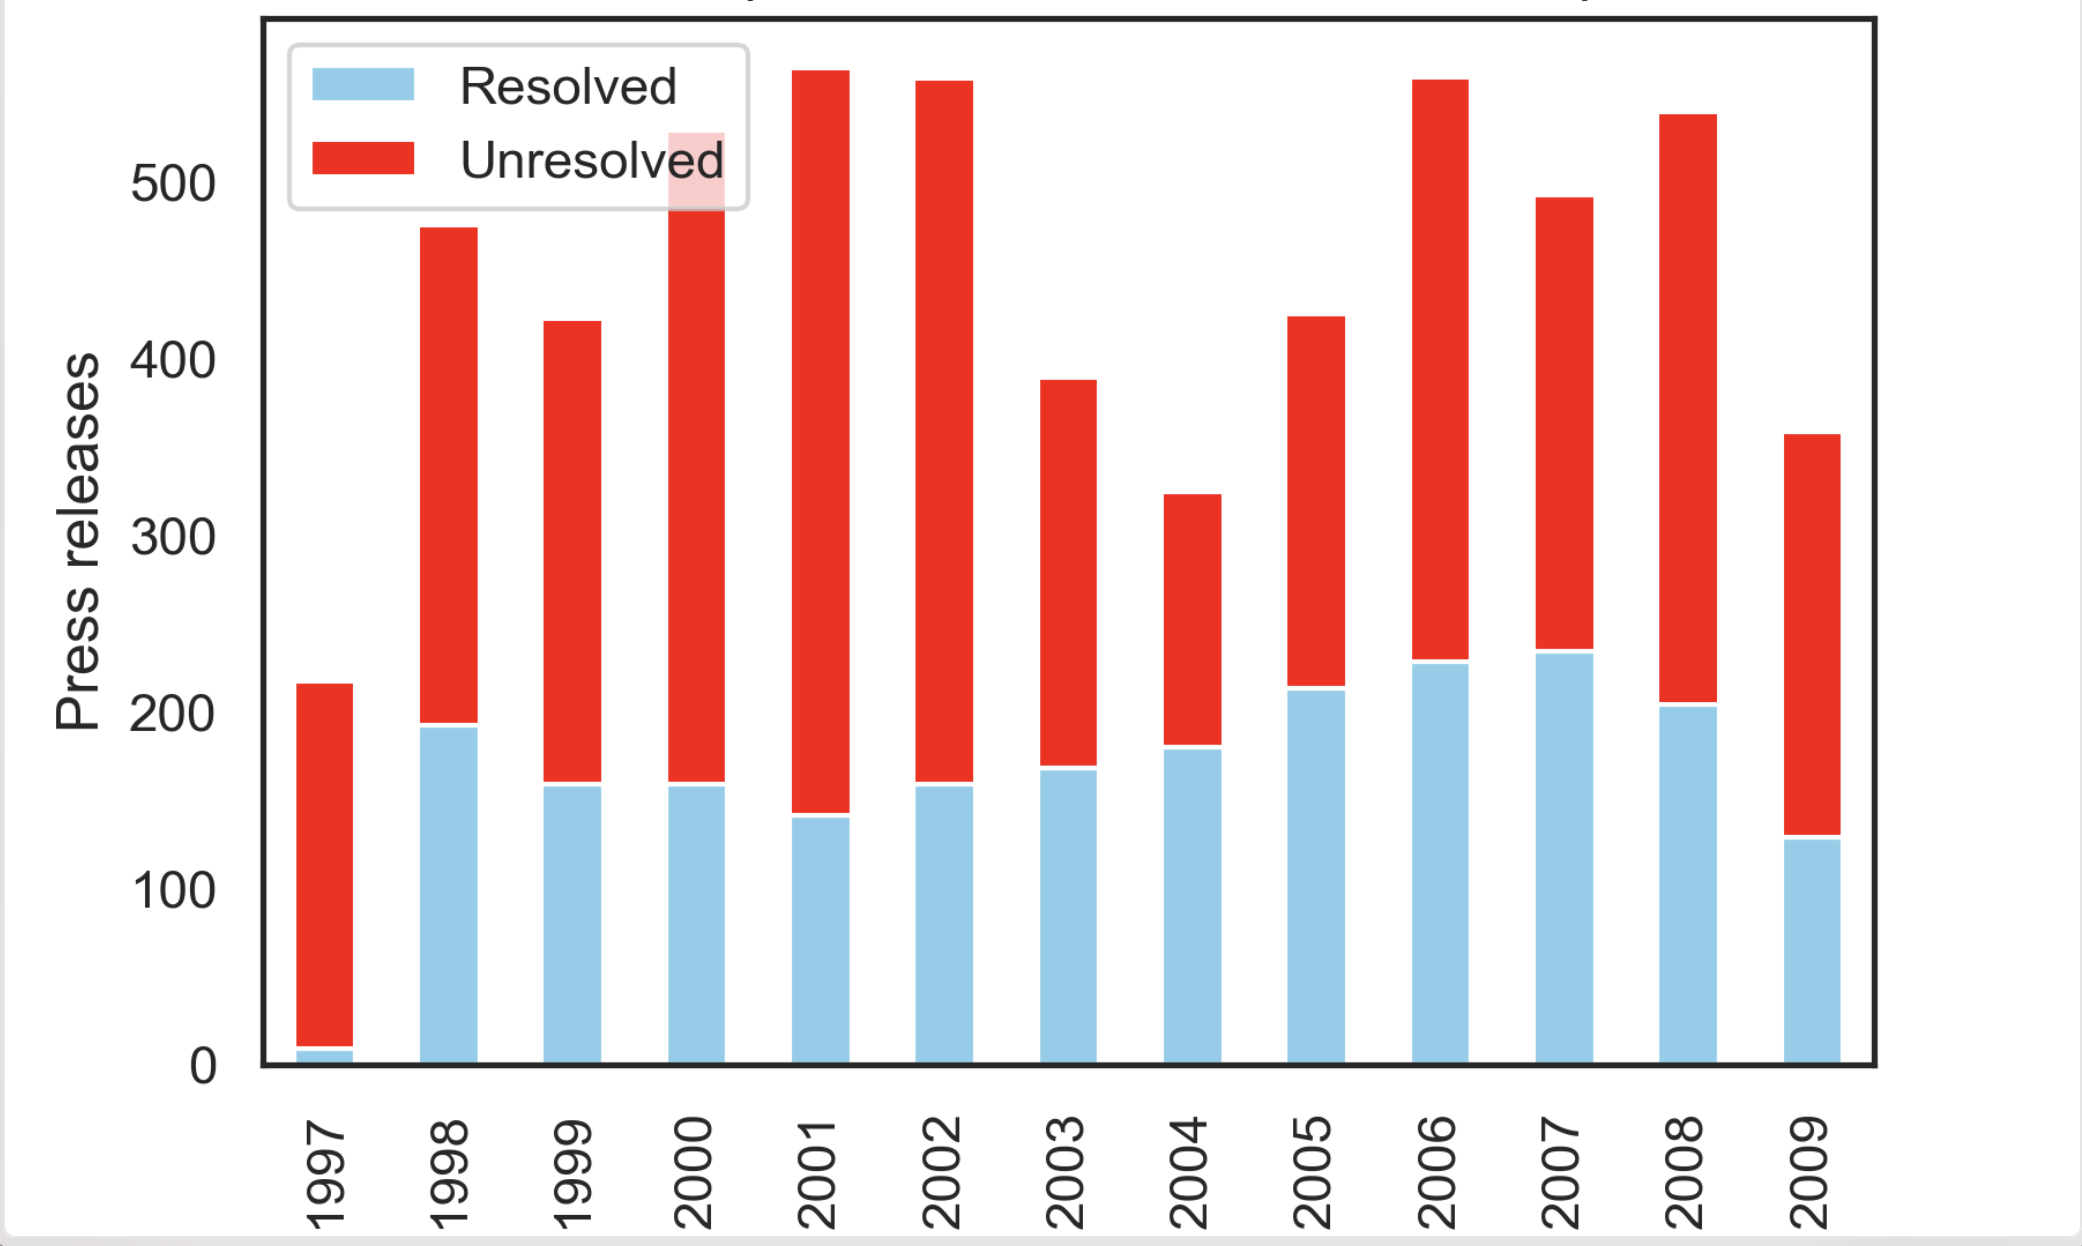
\includegraphics{graphics/linked-unlinked.png}
	\caption{Portion of automatically aligned press releases up to 2009}
	\label{fig:linked-unlinked}
\end{figure}

Since the year 2009 contains both \enquote{linked} and \enquote{unlinked} releases, the script \texttt{split\_2009.py} will split the data accordingly. 
It uses a very simple heuristic: if the file ID of a press release is longer than 5 digits, it is a linked press releases.

\subsubsection{Aligned corpus}
The aligned press releases are saved again to JSON files, with each entry in the file containing the three press releases in the three languages, along with metadata such as date and file ID. 
In the rare case that one language is missing, i.e., the press releases wasn't translated into that language for some reason, it is simply left blank. 
Press releases that are available only in one language are discarded from the aligned corpus.

The script \texttt{create\_corpus.py} deals with this task.
Using the Python library Pandas\footnote{\url{https://pandas.pydata.org}}, the JSON files are read into a DataFrame (a two-dimensional, table-like data structure). 
For linked releases, all the unique ID's are queried, and then for each ID the three languages are collected and saved into a new row. 
The dates are converted from their original format (DD.MM.YY) to an ISO-8601 format (YYYY-MM-DD) \autocite{enwiki:1095673391} for better compatibility and easier processing later.

For JSON files containing unlinked documents, the script \texttt{create\_corpus} has to be run with the switch \texttt{-{}-by-date}, which tells the program to use the date for aligning the documents instead of the file ID.

For an example of the resulting JSON files, with each row containing the aligned documents, see Listing~\ref{lst:json-aligned}.
\begin{lstlisting}[caption={Example for a JSON file containing aligned documents}, captionpos=b, label=lst:json-aligned, language=json]
{
    "0": {
        "id": "2010010501",
        "date": "2010-01-05",
        "DE_title": "Neues Online-Angebot für das Bündner Rechtsbuch",
        "DE_content": " Das im Internet verfügbare Bündner Rechtsbuch ist neu gestaltet worden und enthält neue Funktionalitäten. ...",
        "IT_title": "Nuova offerta online per la Collezione sistematica del diritto cantonale grigionese",
        "IT_content": " La Collezione sistematica del diritto cantonale grigionese disponibile in internet è stata ristrutturata e contiene nuove funzioni. ... ",
        "RM_title": "Nova purschida d'internet per il cudesch da dretg grischun",
        "RM_content": " Il cudesch da dretg grischun che stat a disposiziun en l'internet ha survegnì in nov concept e novas funcziuns. ... "
    },
    "1": {
        "id": "2010010502",
        "date": "2010-01-05",
        "DE_title": "Staupe bei Füchsen und Dachsen im Puschlav",
        "DE_content": " Nachdem sich im Verlaufe des letzten Herbstes die Staupe-Krankheit bei Wildtieren in Nord- und Mittelbünden verbreitete, sind im Laufe der letzten Wochen nun auch im Puschlav bei Füchsen und Dachsen Infektionen mit dem Staupevirus nachgewiesen worden. ... ",
        "IT_title": "Volpi e tassi affetti da cimurro in Valposchiavo",
        "IT_content": " Dopo che nel corso dell'autunno il cimurro si è diffuso tra gli animali selvatici del Grigioni settentrionale e centrale, nelle ultime settimane la presenza del virus è stata rilevata anche tra volpi e tassi della Valposchiavo. ...  ",
        "RM_title": "Pesta dals chauns tar vulps e tar tass en il Puschlav",
        "RM_content": " Suenter che la pesta da chauns è sa derasada tar la selvaschina dal Grischun dal nord e central en il decurs da l'atun passà, èn vegnidas cumprovadas en il decurs da las ultimas emnas ussa er infecziuns cun il virus da questa malsogna tar vulps e tar tass en il Puschlav. ... "
    },
    "2": {
        "id": "2010010801",
        "date": "2010-01-08",
        "DE_title": "Projekt Sicherheitsfunknetz POLYCOM Graubünden mit Vertragsunterzeichnung offiziell gestartet",
        "DE_content": " Die Vorsteherin des Departements für Justiz, Sicherheit und Gesundheit, Regierungsrätin Barbara Janom Steiner, und der Chef des Grenzwachtkorps, Jürg Noth, haben heute in Chur eine Vereinbarung zur Realisierung des Sicherheitsfunknetzes POLYCOM im Kanton unterzeichnet. ... ",
        "IT_title": "Avviato ufficialmente con la sottoscrizione del contratto il progetto di rete radio di sicurezza POLYCOM Grigioni",
        "IT_content": " La Consigliera di Stato Barbara Janom Steiner, direttrice del Dipartimento di giustizia, sicurezza e sanità, e il capo del Corpo delle guardie di confine, Jürg Noth, hanno sottoscritto oggi a Coira un accordo per la realizzazione nel Cantone della rete radio di sicurezza POLYCOM. ... ",
        "RM_title": "Il project per la rait radiofonica da segirezza POLYCOM dal Grischun è vegnì lantschà uffizialmain cun suttascriver il contract",
        "RM_content": " La scheffa dal departament da giustia, segirezza e sanadad, cussegliera guvernativa Barbara Janom Steiner, ed il schef dal corp da guardias da cunfin, Jürg Noth, han suttascrit oz a Cuira ina cunvegna per realisar la rait radiofonica da segirezza POLYCOM en il chantun. ... "
    },
}
\end{lstlisting}

% \section{Manual alignment of unlinked documents}
% As can be seen in figure~\ref{fig:linked-unlinked}, a big portion of the unlinked documents cannot be automatically aligned using the simple heuristic described in section~\ref{sec:linked-unlinked}. 
% To deal with that, the script \texttt{create\_corpus.py} will write the titles and file IDs of all the discarded documents to a CSV file, one for each year. 

% These CSV files can be used for manually aligning the corresponding documents. 
% This is done by enumerating the documents while using the same digit for corresponding documents. 
% The CSV files containing the now enumerated documents can be given to the script \texttt{create\_corpus.py} using the argument \texttt{add-from-csv} to combine the enumerated documents as linked documents into the JSON file.

\section{SQLite database}
The query language SQL offers flexible and complex way to query databases. 
For this reason, I decided to save the resulting corpus in an SQLite database. 
I opted for SQLite because it doesn't require running a separate server and SQLite databases can be easily built, edited and accessed using \texttt{sqlite3}\footnote{\url{https://docs.python.org/3/library/sqlite3.html}}, a Python module delivered with the Python standard library\footnote{\url{https://docs.python.org/3/tutorial/stdlib.html}}.

The SQLite database contains two tables, \texttt{corpus} and \texttt{raw} with the exact same structure as the two JSON files described in Listings~\ref{lst:json} and \ref{lst:json-aligned}.

The final result is an SQLite database (\texttt{corpus.db}) containing two tables:
\begin{itemize}
	\item \texttt{corpus}: all the aligned documents from 1997 until today, see Table~\ref{tab:corpus.db-corpus} for details.




	% \begin{itemize}
	% 	\item id: Automatically incremented unique ID
	% 	\item file\_id: Original file ID
	% 	\item date: Release date
	% 	\item DE\_title: Title of German document
	% 	\item DE\_content: Content of German document
	% 	\item IT\_title: Title of Italian document
	% 	\item IT\_content: Content of Italian document
	% 	\item RM\_title: Title of Romansh document
	% 	\item RM\_content: Content of Romansh document
	% \end{itemize}
	\item \texttt{raw}: All the documents contained in the HTML files scraped from the website. 
	See Table~\ref{tab:corpus.db-raw} for details. 
% 	The rows contain the following columns:
% 	\begin{itemize}
% 		\item id: Automatically incremented unique ID
% 		\item file\_id: Original file ID
% 		\item orig\_file: Original filename
% 		\item lang: Document language (\texttt{DE} for German, \texttt{IT} for Italian, \texttt{RM} for Romansh)
% 		\item title: Document title
% 		\item date: Release date
% 		\item content: Document content
% 	\end{itemize}
% \end{itemize}
\end{itemize}


\begin{table}
\centering
\begin{tabular}{lp{7cm}}
\toprule
Column & Description \\
\midrule
	\texttt{id} & Automatically incremented unique ID \\
	\texttt{file\_id} & Original file ID \\
	\texttt{date}&  Release date \\
	\texttt{DE\_title} &  Title of German document \\
	\texttt{DE\_content} &  Content of German document \\
	\texttt{IT\_title} &  Title of Italian document \\
	\texttt{IT\_content} &  Content of Italian document \\
	\texttt{RM\_title} &  Title of Romansh document \\
	\texttt{RM\_content} &  Content of Romansh document \\
\bottomrule
\end{tabular}
\caption{Description of the table \texttt{corpus} in \texttt{corpus.db}}
\label{tab:corpus.db-corpus}
\end{table}


\begin{table}
\centering
\begin{tabular}{l p{7cm}}
\toprule
Column & Description \\
\midrule
		\texttt{id} & Automatically incremented unique ID \\
		\texttt{file\_id} &  Original file ID \\
		\texttt{orig\_file} & Original filename \\
		\texttt{lang} &  Document language (\texttt{DE} for German, \texttt{IT} for Italian, \texttt{RM} for Romansh) \\
		\texttt{title} &  Document title \\
		\texttt{date} & Release date \\
		\texttt{content} &  Document content \\
\bottomrule
\end{tabular}
\caption{Description of the table \texttt{raw} in \texttt{corpus.db}}
\label{tab:corpus.db-raw}
\end{table}

% \footnotetext{I opted for SQLite instead of mySQL since SQLite does not require installing any special software or running a server locally. The Python library sqlite3 is shipped with Python as a standard package.}

\section{Summary}
For compiling the corpus, the following steps were taken:
\begin{enumerate}
	\item Scrape website and save HTML documents locally
	\item Extract relevant content from HTML files (date, language, title and content) and save to JSON files
	\item Read the JSON files using Pandas DataFrames, align the documents and save to new JSON files
	\item Feed both types of JSON files into an SQLite database
\end{enumerate}


\subsection{Statistics}
The corpus contains \numprint{3536} parallel documents, with a yearly average of 56.8 documents prior to 2009 and a yearly average of 207.8 documents from 2009 onward\footnote{Not including 2022}. 
See also Table~\ref{tab:docs-per-year}. Table~\ref{tab:docs-per-lang} breaks down the number of documents per each year and language. 

The corpus contains \numprint{2484250} German tokens, \numprint{2760690} Romansh tokens and \numprint{2581168} Italian tokens\footnote{Punctuation included}. Table~\ref{tab:top-20} displays the 20 most frequent tokens for each language in the corpus.

\begin{table}
\centering
\begin{tabular}{cc|cc}
\toprule
Year & Documents & Year & Documents\\
\midrule
1997 &	3 & 2010	&184\\
1998 & 64 & 2011	&167\\
1999 & 53 & 2012&	207 \\
2000 & 53 & 2013 &	219 \\
2001 &	47 &2014	&218\\
2002 & 53 &2015	&183 \\
2003 &	56 & 2016	&190\\
2004&	60 & 2017	&207\\
2005	&71 & 2018	&221 \\
2006	&76 & 2019	&216 \\
2007	&78 & 2020	&286 \\
2008	&68 & 2021	&294 \\
2009	&109&2022	&153\\
		
		\midrule
		&   & \textbf{Total} & \textbf{\numprint{3536}} \\
\bottomrule
\end{tabular}
\caption{Number of parallel documents per year, as of July 20, 2022.}
\label{tab:docs-per-year}
\end{table}

\begin{table}
\centering
\begin{tabular}{cccc}
\toprule
Year & German & Romansh & Italian\\
\midrule
1997 & 181 & 17 & 18\\ 
1998 & 168 & 153 & 153\\ 
1999 & 161 & 130 & 130\\ 
2000 & 192 & 167 & 169\\ 
2001 & 233 & 159 & 171\\ 
2002 & 235 & 157 & 165\\ 
2003 & 167 & 110 & 111\\ 
2004 & 132 & 97 & 94\\ 
2005 & 157 & 134 & 133\\ 
2006 & 211 & 173 & 174\\ 
2007 & 199 & 147 & 145\\ 
2008 & 201 & 168 & 169\\ 
2009 & 212 & 175 & 176\\ 
2010 & 219 & 183 & 184\\ 
2011 & 203 & 167 & 167\\ 
2012 & 254 & 207 & 207\\ 
2013 & 260 & 219 & 219\\ 
2014 & 260 & 218 & 218\\ 
2015 & 227 & 183 & 183\\ 
2016 & 221 & 190 & 190\\ 
2017 & 236 & 207 & 207\\ 
2018 & 248 & 221 & 220\\ 
2019 & 238 & 216 & 216\\ 
2020 & 310 & 284 & 285\\ 
2021 & 322 & 294 & 294\\ 
2022 & 169 & 153 & 153\\
\midrule
\textbf{Total} & \textbf{5616}	&\textbf{4529}&	\textbf{4551}\\
\bottomrule
\end{tabular}
\caption{Number of documents per language and year as of 20 July, 2022.}
\label{tab:docs-per-lang}
\end{table}


\begin{table}
\centering
\begin{tabular}{lc|lc|lc}
\toprule
\multicolumn{2}{c|}{German} &  \multicolumn{2}{c|}{Romansh} & \multicolumn{2}{c}{Italian} \\
Type & Count & Type & Count & Type & Count\\
\midrule
.	&	122176	&	da	&	199663	&	di	&	110946 \\ 
,	&	88048	&	la	&	111803	&	.	&	93732 \\ 
der	&	82288	&	.	&	98181	&	,	&	80509 \\ 
und	&	74298	&	,	&	59456	&	e	&	62295 \\ 
die	&	69741	&	e	&	56493	&	la	&	40558 \\ 
in	&	33423	&	il	&	50155	&	il	&	38844 \\ 
für	&	31464	&	per	&	46475	&	per	&	38100 \\ 
des	&	27467	&	las	&	45869	&	del	&	36805 \\ 
den	&	27037	&	en	&	42061	&	della	&	31309 \\ 
:	&	26154	&	dal	&	40407	&	a	&	31164 \\ 
Die	&	25310	&	a	&	30284	&	in	&	30506 \\ 
von	&	25205	&	ils	&	22554	&	dei	&	25525 \\ 
im	&	20684	&	:	&	21442	&	:	&	21407 \\ 
Graubünden	&	17859	&	cun	&	20114	&	un	&	20410 \\ 
zu	&	17709	&	che	&	19931	&	i	&	17909 \\ 
werden	&	17258	&	La	&	18494	&	è	&	17525 \\ 
mit	&	16621	&	ina	&	18413	&	le	&	17051 \\ 
Regierung	&	15557	&	è	&	18053	&	che	&	15986 \\ 
auf	&	15276	&	Grischun	&	16775	&	Governo	&	15592 \\ 
das	&	14370	&	ed	&	16030	&	Grigioni	&	15337 \\ 
\bottomrule 
\end{tabular}
\caption{Twenty most frequent tokens in each language in the corpus.}
\label{tab:top-20}
\end{table}

